\section{Case Study: Web eID}

Released in the Summer of 2021 \cite{ria-webeid} and having undergone significant changes in January of 2022, this eID solution allows users to authenticate and sign documents using their country's smart cards.

Functionally this software solution is split into three parts: software the user needs to install on their computer, a javascript library that acts as a data transfer intermediary, and the certificate validation library for the back-end.

The software users need to install is similar to the one various countries' governments issue. The significant difference is that this software supports more than one country's eID solutions. Supported countries include Estonia, Latvia, Lithuania, and Finland \cite{ria-webeid}.

This service is built by the Estonian Information System Authority.

\subsection{Authentication Protocol}

Figure \ref{fig:web-eid-authentication} displays the high-level overview of the complete flow of data within the Web eID system. A detailed explanation of the steps can be found in the technical specification \cite{ria-webeid-systemarchitecture}. Companies implementing the framework should only pay attention to the browser and the server application (steps 1-3 and 13-17).

\begin{figure}
  \centering
  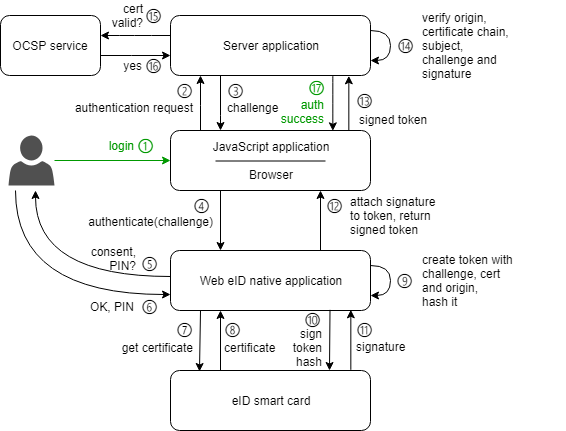
\includegraphics[scale=0.6]{webeid/Web-eID-authentication-communication-diagram}
  \caption{Web eID Authentication flow \cite{ria-webeid-systemarchitecture}}
  \label{fig:web-eid-authentication}
\end{figure}

\subsection{Trust Anchor}

Unlike Dokobit and eeID, Web eID does not provide any guarantees about the trustworthiness of a certificate. It requires the relying party to manually verify the received identity certificate \cite{ria-webeid-source-web-eid-authtoken-validation-java-readme}. The verification process involves checking the origin, certificate expiry, trust chain, OCSP response, and the signed challenge token.

One advantage of using Web eID is that there are no third-party intermediate services, which reduces the number of potential attack vectors, making it theoretically more secure than both eeID and Dokobit. The identity information comes directly from the device storing it. This benefit, however, comes with a comparatively massive implementation and maintenance cost, as the developers would have to create and maintain the trusted certificate store.

\subsection{Pricing}

The eID solutions enabled by Web eID software are free of charge to use, as the only external validation required, the OCSP \cite{rfc6960} requests, are free.

\subsection{Security Requirements}

The data flow used by Web eID is fundamentally different from the used by the other two eID solutions. The main difference is that the server should not trust the identity information received from the eID provider. This difference makes using the IETF guidelines document \cite{ietf-oauth-security-topics-19} less valuable as it does not cover the case of what to do when the identity information is not trusted. Fortunately, RIA provides an exceptional integration and hardening guide \cite{ria-webeid-systemarchitecture}, which we will use for our analysis.

\paragraph{Communication channel}

The Web eID framework is the only one covered by this thesis that uses an insecure communication channel. The reason why is it not secure is because the user or user agent can freely modify the identity data they send to the relying party. Developers must take caution and verify received data when integrating this eID solution. This channel is highly susceptible to man-in-the-middle, forgery, or other attacks done by a malicious end user.

\subsubsection{Requirements for the Identity Provider}

In Web eID's case, the identity provider is the Javascript library and the software used to bridge the connection between the library and the smart cards. Because the library can and should be embedded into the log-in page, the user is not required to leave the company's website.

Additionally, because the identity provider is on the same website as the relying party, it does not make sense to discuss the requirements separately, as was the case for eeID and Dokobit. For this reason, we will cover all common protocol attacks in the next section.

\subsubsection{Requirements for the Relying Party}

Web eID does not have a hosted website to verify security of. Instead, we will check if the integration documentation covers all common attacks.

\paragraph{Replay attacks}

\begin{itemize}
  \item The protocol requires the server to send a \texttt{challenge nonce} to the Web eID software.
  \item This generated \texttt{nonce} must be between 32 and 96 bytes (inclusive) in length \cite{ria-webeid-source-web-eid-app-authenticate}.
\end{itemize}

The software allows for the use of nonces more than once. It is the server's responsibility to create nonces; make sure that they were not already used or expired.

The documentation states this explicitly: "Cache must be used for protection against replay attacks by guaranteeing that each authentication token can be used exactly once" \cite{ria-webeid-source-web-eid-authtoken-validation-java-readme}.

\paragraph{Insufficient Redirect URI Validation}

\begin{itemize}
  \item When signing the \texttt{challenge nonce}, the Web eID library hashes and signs {location.origin} variable in addition to the \texttt{nonce}.
\end{itemize}

While not entirely redirect URI validation, the protocol still requires the domain check to mitigate against man-in-the-middle and authentication token export and replay attacks \cite{ria-webeid-systemarchitecture}.

\paragraph{Cross-Site Request Forgery}

\begin{itemize}
  \item Documentation requires that "Cookie-based authentication must be protected against cross-site request forgery (CSRF) attacks and extra measures must be taken to secure the cookies by serving them only over HTTPS and setting the HttpOnly, Secure and SameSite attributes" \cite{ria-webeid-source-web-eid-authtoken-validation-java-readme}.
\end{itemize}

The document does not specify how companies should prevent CSRF, only that they must. However, the documentation does come with a comprehensive implementation example the developers can use as a reference.

\paragraph{Certificate injection}

Web eID, unlike the eID solutions analyzed before, comes with a hazardous problem. The client has complete control over the certificate they send and, if the certificate is not sufficiently validated, has the potential to impersonate anyone. Arnis Paršovs demonstrated an exploit of a similar variety back in 2015 \cite{seb-auth-bypass}. Fortunately, the Web eID documentation provides validation steps the relying party must verify to mitigate this form of attack \cite{ria-webeid-systemarchitecture}:

\begin{enumerate}
  \item the current time falls within the authentication certificate's validity period;
  \item the purpose of the authentication certificate's key usage is client authentication;
  \item the authentication certificate does not contain any disallowed policies;
  \item the authentication certificate is signed by a trusted certificate authority;
  \item certificate is not revoked (OCSP);
  \item signed \texttt{challenge nonce} corresponds to the certificate's public key.
\end{enumerate}

The documentation is thorough, listing all requirements developers must take to harden their systems. Additionally, documentation also provides reasons for the requirements' inclusion. Unfortunately, this list of validations is far longer than the other two eID solutions mentioned earlier, making it more challenging to integrate.

\subsection{Integration}

For each protocol implementation step, developers will have to fulfill certain validation requirements before the system goes into production.

\subsubsection{Preparation}

Building the \texttt{challenge nonce}. The goal of these steps is to create the challenge the user will have to sign with their private key. There are a couple of requirements the relying party must satisfy:
\begin{enumerate}
  \item Generated \texttt{challenge nonce} must be between 32 and 96 bytes (inclusive) in length \cite{ria-webeid-source-web-eid-app-authenticate};
  \item It must be guaranteed that the authentication token is received from the same browser to which the corresponding \texttt{challenge nonce} was issued \cite{ria-webeid-source-web-eid-authtoken-validation-java-readme}. The eID solution creators suggest attaching it to the user session.
  \item Cache must be used for protection against replay attacks by guaranteeing that each authentication token can be used exactly once \cite{ria-webeid-source-web-eid-authtoken-validation-java-readme}.
\end{enumerate}

In the implementation example, these measures were addressed by:
\begin{enumerate}
  \item a 64 byte cryptographically secure randomly generated \texttt{nonce} is created (see Listing \ref{lst:web-eid-challenge});
  \item \texttt{challenge nonce} is set in the user's session, which adversaries cannot access or tamper;
  \item the generated \texttt{nonce} is stored into local memory cache for later use; \texttt{nonce} expires after 5 minutes;
  \item an input field is rendered on the page with a unique CSRF validation token, which prevents cross-site request forgery attacks (see Listing \ref{lst:web-eid-challenge-ui});
\end{enumerate}

\begin{lstlisting}[caption={Web eID Challenge Endpoint}, label={lst:web-eid-challenge}]
private TimeSpan ChallengeLifetime { get; } = TimeSpan.FromMinutes(5);

private readonly IMemoryCache _cache; // Injected

[HttpGet("challenge")]
public IActionResult GetChallenge()
{
    var nonce = RandomNumberGenerator.GetBytes(64);

    _cache.Set(Convert.ToBase64String(nonce), true, ChallengeLifetime);
    HttpContext.Session.Set("eid.challenge", nonce);

    return Ok(new { nonce });
}
\end{lstlisting}


\begin{lstlisting}[caption={Web eID UI excerpt}, label={lst:web-eid-challenge-ui}, language={html}]
@inject Microsoft.AspNetCore.Antiforgery.IAntiforgery _csrf
@{ var csrfToken = _csrf.GetAndStoreTokens(HttpContext); }

<!-- Button used to sign in -->
<a role="button" class="btn btn-secondary" id="webeid-auth-button">Web eID</a>

<input id="csrfToken" type="hidden" value="@csrfToken.RequestToken"/>

<script>
    ...

    const authTokenResponse = await fetch("/signin-id/login", {
        method: "POST",
        headers: {
            "Content-Type": "application/json",
            "RequestVerificationToken": document.getElementById("csrfToken").value
        },
        body: JSON.stringify(...)
    });

    ...
</script>
\end{lstlisting}

\subsubsection{Validation}

After the user signs the \texttt{nonce} challenge and sends their certificate, the server must verify its authenticity. The application must perform all of the following before allowing the user to sign in:

\begin{enumerate}
  \item verify the CSRF token from earlier steps \cite{ria-webeid-source-web-eid-authtoken-validation-java-readme};
  \item verify the \texttt{challenge nonce} came from the original user and has not expired, was not consumed;
  \item verify the certificate validity and check if \texttt{nonce} was signed by the associated private key (see below);
  \item issue an authentication token with the fields from the certificate's subject;
\end{enumerate}

In our implementation, these measures were addressed by:
\begin{enumerate}
  \item the back-end endpoint for log-in is decorated with \texttt{ValidateAntiForgeryToken} attribute. This attribute instructs the ASP.NET API to ignore requests not containing a CSRF token \cite{msdocs-anti-request-forgery}. A JavaScript application can only access the protected endpoints by providing \texttt{RequestVerificationToken} header (see Listing \ref{lst:web-eid-challenge-ui});
  \item the application tries to extract the \texttt{challenge nonce} from the browsing session. The process would succeed if the session cookie were not modified. After the extraction, the application checks the \texttt{nonce} cache to verify if the challenge is still active. Cache hit means the \texttt{nonce} has not expired, and no previous authentication attempt was performed. Remove the \texttt{challenge nonce} from all stores.
  \item The API calls a standalone validation service to verify the \texttt{nonce} and certificate (see certificate and \texttt{nonce} verification section below).
  \item Application populates the ASP.NET identity management system with the fields from the certificate: serial number, given name, surname, country. An identity session cookie is sent to the client.
\end{enumerate}

\begin{lstlisting}[caption={Web eID Login Endpoint}, label={lst:web-eid-login}]
[HttpPost("login")]
[ValidateAntiForgeryToken]
public async Task<IActionResult> Login([FromBody] WebIdAuthTokenResponse token)
{
    // Obtain the challenge from session
    if (!HttpContext.Session.TryGetValue(ChallengeNonceKey, out var nonce) && nonce == null)
        return Unauthorized();

    // Check if token was not used before or expired
    var challenge = Convert.ToBase64String(nonce);
    if (!_cache.TryGetValue(challenge, out _))
        return Unauthorized();

    _cache.Remove(challenge);
    HttpContext.Session.Remove(ChallengeNonceKey);

    // Validate the certificate and signed challenge
    var validationResult = await _webEidValidationService.GetResult(new WebEidValidationRequest(token, nonce));
    if (!validationResult.Success)
        return Forbid();

    // Certificate is valid. Sign in the user

    await HttpContext.SignInAsync(BuildUser(new X509Certificate2(Convert.FromBase64String(token.UnverifiedCertificate)).Subject));

    return Ok();
}
\end{lstlisting}

\subsubsection{Certificate and Challenge Verification}

This step is the most complicated in the entire validation process. To prevent any issues with incorrect implementation, the framework maintainers recommend using their library for validation \cite{ria-webeid-source-web-eid-authtoken-validation-java-readme}. Libraries can come with security vulnerabilities, and developers are reluctant to update their used version; however, it is still more favorable than to create vulnerabilities from misconfiguration \cite{9240619}.

The eu.webeid.security Java package performs most of the certificate validation: expiry, purpose, policy, OCSP \cite{ria-webeid-source-web-eid-authtoken-validation-java-readme}. Developers will only have to configure the CA and host validation. Configuration is handled by providing a set of trusted CA certificates for trust chain verification and the hostname for challenge nonces (see Listing \ref{lst:web-eid-java-lib}).

\begin{lstlisting}[caption={Web eID Login Endpoint}, label={lst:web-eid-java-lib}]
public class AuthTokenValidatorService {

  @Bean
  public AuthTokenValidator validator() {
    try {
      return new AuthTokenValidatorBuilder()
        .withSiteOrigin(URI.create(System.getenv("ORIGIN_URL")))
        .withTrustedCertificateAuthorities(loadTrustedCACertificatesFromCerFiles())
        .build();
    } catch (JceException e) {
      throw new RuntimeException("Error building the Web eID auth token validator.", e);
    }
  }

  private X509Certificate[] loadTrustedCACertificatesFromCerFiles() {
    List<X509Certificate> caCertificates = new ArrayList<>();

    try {
      CertificateFactory certFactory = CertificateFactory.getInstance("X.509");

      File[] files = new File("/certs").listFiles((f, n) -> n.endsWith(".cer"));
      if (files != null) {
        for (File file : files) {
          try (InputStream stream = new FileInputStream(file)) {
            X509Certificate caCertificate = (X509Certificate) certFactory.generateCertificate(stream);
            caCertificates.add(caCertificate);
          }
        }
      }
    } catch (CertificateException | IOException e) {
      throw new RuntimeException("Error initializing trusted CA certificates.", e);
    }

    return caCertificates.toArray(new X509Certificate[0]);
  }
}
\end{lstlisting}

The token validation service described in Listing \ref{lst:web-eid-java-lib} requires WorkAuth maintainers to set the origin URL in the form of an environment variable and to populate the folder \texttt{/certs} with trusted CA certificates.

Origin URL can be obtained by checking the \texttt{window.origin} JavaScript variable in the page containing the log-in button.

For the CA certificate set, the company can get an up-to-date list of trusted certificates at the EU Trust Services Dashboard \cite{eu-trustservices}. The issue with this list is that it contains all trust certificates for various scopes. In our case, we should limit the search to the extent of QCert for ESig. In the case of Estonia and Lithuania, only three entities are certified to issue certificates for QSCD (see Figure \ref{fig:eu-tsp-list}). It is in stark contrast to Spain's 31 \cite{eu-trustservices}. It is possible to further narrow down to only certificate generation services for qualified certificates (CA/QC); however, it would not be possible to narrow down anymore. In the case of Estonia's single TSP, we can see that only 3 CA are currently operational (see Figure \ref{fig:eu-tsp-skid}).

\begin{figure}
  \centering
  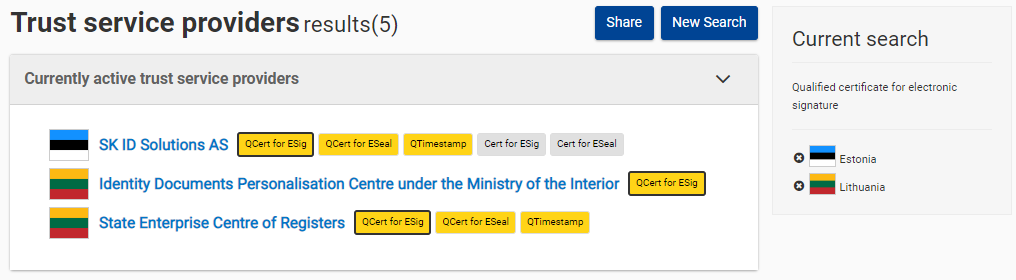
\includegraphics[scale=0.54]{webeid/eu-tsp-search}
  \caption{List of EU Trust service providers of Estonia and Lithuania capable of creating qualified certificates for e-signatures}
  \label{fig:eu-tsp-list}
\end{figure}

\begin{figure}
  \centering
  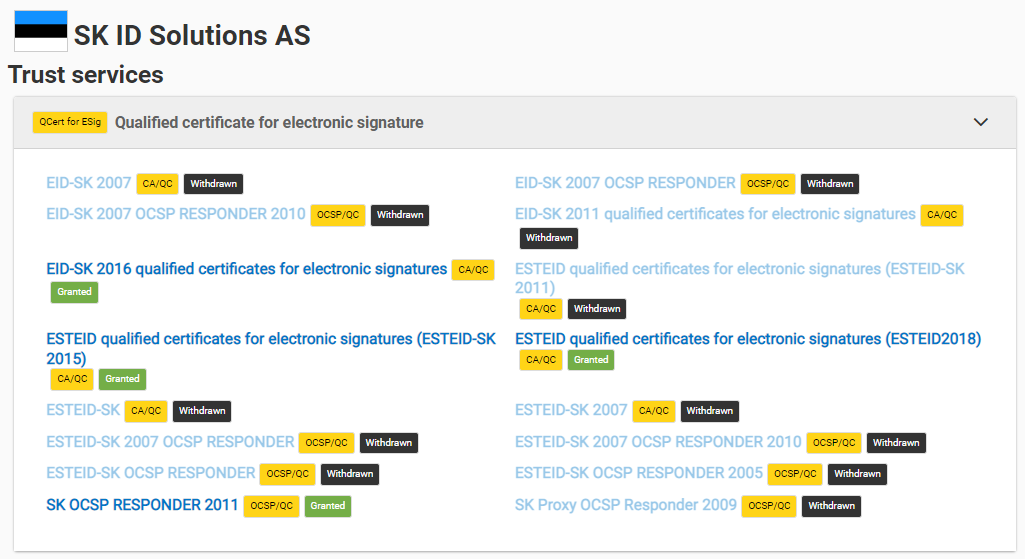
\includegraphics[scale=0.54]{webeid/eu-tsp-skid}
  \caption{List of certificates issued to SK ID Solutions AS for the purposes of Qualified certificate for electronic signature}
  \label{fig:eu-tsp-skid}
\end{figure}

An alternative way to obtain certificates would be to go to the government authority of each country responsible for the distribution of certificates. This action requires prior knowledge of who is responsible for issuing certificates and their purposes.

In Lithuania's case, it is the Ministry of the Interior \cite{eid-lt-ministryofinterior-certificates} who issues two certificates every couple of years. As of early 2022, four certificates are active, and all will be added to the trusted CA list.

In Estonia's case, SK ID Solutions manages the CA certificates \cite{eid-ee-skid-certificates}. Of the three certificates found on the EU Trust Services Dashboard, only two are relevant to us, the 2015 and 2018 ones, as the 2016 one has its purpose for use in Smart-ID, which the Web eID framework does not support.

The final count of certificates is six. Four certificates are required to support Lithuania and two for Estonia. It is essential to keep track of these certificates as each one of them can act as a point of compromise and must be monitored in the event they are revoked for security \cite{roca-vulnerability-lessons-learned} or other issues.

\paragraph{Exposing the service}

With the certificate validation service configured, it is now required to link it to the Web API. If the company orients around using microservices, this service can be just that. All that the validation service requires is to expose an endpoint that accepts a \texttt{nonce} and a token from the JavaScript library and returns a validation result.

Companies must take proper measures to protect such service from adversaries as it acts as a fundamental trust anchor. {Zero trust architecture} \cite{zero-trust-architecture} is an excellent choice for this task.
